\chapter{Besoins non fonctionnels}

\section{Comportement}

\subsection{Performances}
La génération de terrains n'étant pas faite en temps réel, aucune exigence
concernant la vitesse de calcul n'est spécifiée : la qualité du rendu prime sur
le temps d'exécution. Le temps de génération de nos terrains pourra donc \^etre conséquent (de quelques secondes à quelques minutes).\\

Il n'y a pas d'interactivité entre l'utilisateur et le programme pendant l'exécution de ce dernier (le programme peut donc s'exécuter en tâche de fond).\\

\subsection{Facilité d'utilisation}
La bibliothèque devra \^etre facile à prendre en main pour l'utilisateur (qui sera un développeur) et devra proposer un maximum d'algorithmes de génération de terrains (parmis ceux qui sont décrits dans les besoins fonctionnels).\\

Il s'agit de développer une bibliothèque et non un logiciel. L'utilisateur
de notre projet est donc un développeur. En conséquence il n'est pas demandé
d'implémenter d'interface graphique pour l'utilisation de la bibliothèque elle-m\^eme, l'utilisateur final pourra, s'il le souhaite, en créer une en s'appuyant sur les différents services proposés par notre bibliothèque.\\

\subsubsection{Contraintes}
Une documentation devra être livrée avec la bibliothèque.

\subsubsection{Validation}
Plusieurs programmes d'exemples illustrant l'utilisation de notre bibliothèque seront livrés.

\subsection{Portabilité}
La bibliothèque sera développée pour les plateformes Linux/x86 et devra utiliser
GNU Autotools comme système de construction.

\subsubsection{Contraintes}
Toute utilisation de bibliothèque devra \^etre justifiée afin d'éviter la prolifération des dépendances. La bibliothèque boost ne devra \^etre utilisée qu'en cas d'absolue nécessité.

\subsection{Persistance des données de la génération procédurale}
Les exécutions avec les mêmes paramètres (méthodes, graine aléatoire, etc)
doivent fournir le même résultat.

\subsubsection{Validation}
Pour N exécution d'une méthode avec des paramètres identiques, comparer les cartes d'élévations obtenues (sommet par sommet) en vérifiant que les sommets aient les mêmes élévations. 

\section{Besoins organisationnels}

\subsection{Standards, processus de développement}

\subsubsection{Langage}
L'implémentation sera faite en C++11, la version standard actuelle de C++ depuis
2011.

\subsubsection{Style de codage}
Le projet devra respecter le style de codage de linux :\\
\url{https://www.kernel.org/doc/Documentation/CodingStyle}\\
\emph{(Dernière visite : 10/02/2014)}
%\subsection{Gestion du temps}
%% TODO diagramme Gant

\section{Autres besoins}
\subsection{Contraintes légales}
Le projet sera distribué sous Licence Publique Générale Limitée GNU (GNU LGPL).

Nous avons choisi cette licence car c'est une licence de logiciel libre mais
moins contraignante que la GPL. En effet elle autorise à lier un programme
développé sous cette licence à du code non (L)GPL. Il sera donc possible d'utiliser notre bibliothèque dans un programme publié sous une autre licence sans révoquer celle-ci.

\subsection{Contraintes d'interopérabilité}
Les cartes d'élévation produites par notre bibliothèque devront être lisible par les visualisateurs
 suivants : TerraGen 3 et Blender 3D.\\
\textbf{Terragen 3} utilise des fichiers au format .TER et les modélise sous forme de terrains.\\
Pour \textbf{Blender 3D}, les traitements en amont sont plus simples car ce logiciel charge
une carte d'élévation (image en niveaux de gris) et sous forme de modèle (fichiers
.obj).
Les configurations se font ensuite depuis Blender 3D.


\chapter{Faisabilité}
\section{Estimation de la taille mémoire requise pour les cartes d'élévations}
La figure~\ref{fig:heightmap_memory} illustre la taille mémoire requise pour
stocker les cartes d'élévations en fonction de leurs tailles et du type des entiers
utilisés. Pour permettre plus de lisibilité le graphique utilise une échelle
logarithmique.\\

\begin{figure}[!ht]
    \begin{center}
        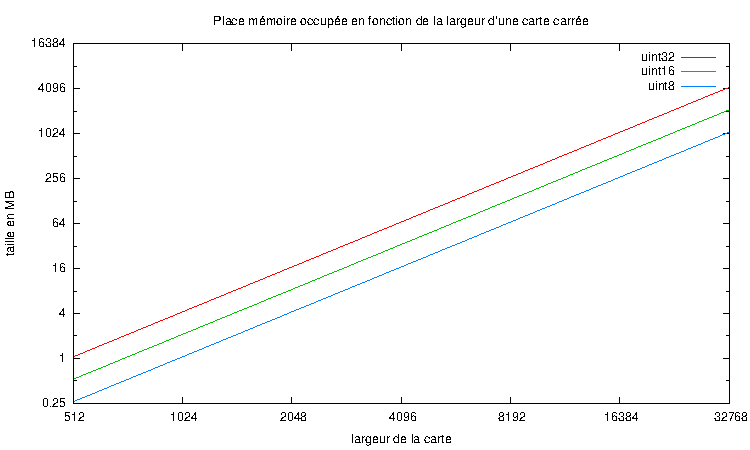
\includegraphics[width=15cm]{resources/heightmap-memory.pdf}
        \label{fig:heightmap_memory}
        \caption{taille mémoire occupée par une carte d'élévations}
    \end{center}
\end{figure}

\begin{itemize}
\item si l'on utilise des entiers non signés sur 8 bits (uint8), les valeurs
possibles pour les élévations s'étalent de 0 à 255, cet intervalle est assez
restrictif et limite la précision de la carte.

Cependant la place occupée en mémoire est faible (environ 256 Mo pour une carte
carrée de largeur 16 384) ;\\

\item si l'on utilise des entiers non signés sur 16 bits (uint16), les valeurs
possibles pour les élévations s'étalent de 0 à 65 535, cet intervalle est tout à
fait suffisant pour produire des carte ayant un niveau de détail élevé.

De plus la place occupée en mémoire est acceptable (environ 512 Mo pour une carte
carrée de largeur 16 384) ;\\

\item si l'on utilise des entiers non signés sur 32 bits (uint32), les valeurs
possibles pour les élévations s'étalent de 0 à 4 294 967 295, cet intervalle est
démesurément grand et n'est pas nécessaire pour produire des carte ayant un
niveau de détail élevé.

De plus la place occupée en mémoire est importante (environ 1 Go pour une carte
carrée de largeur 16 384).
\end{itemize}